\documentclass{report}
\usepackage{graphicx}
\usepackage{amssymb}
\usepackage{amsmath}
\title{Calcolo differenziale}

\begin{document}
\maketitle
\tableofcontents

\newpage
\section{Equazioni e disequazioni}
    \subsection{La retta}
        \begin{center}
            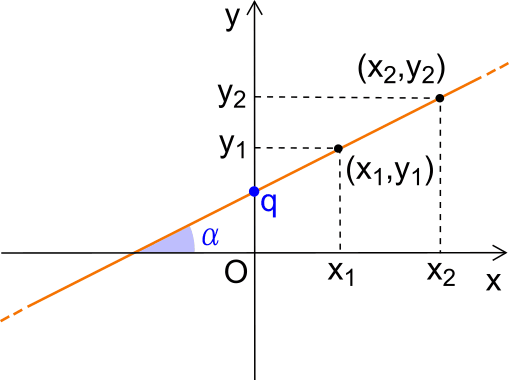
\includegraphics[width=\textwidth]{retta.png}
        \end{center}
        La retta è \textbf{lineare} in x e y. \\
        Se $ m > 0 $ è \textbf{crescente}, se $ m < 0 $ è \textbf{decrescente}.
        \textbf{Forma esplicita} $ y = mx + q $. \\
        Questa forma descrive tutte le rette tranne quella \textbf{verticale}: $ y = c $ \\
        \textbf{Forma implicita} $ ax + by + c = 0 $
        $$ m = tg\Theta = \frac{\Delta y}{\Delta x} $$
        $$ y = m(x - x_0) + y_0 \Longleftrightarrow q = y_0 - mx_0 $$
        $$ ax \geq -b \Longrightarrow $$
        \begin{itemize}
            \item se $a > 0: x \geq \frac{-b}{a} $
            \item se $a < 0: x \leq \frac{-b}{a} $
        \end{itemize}
    \subsection{Polinomi di secondo grado: le parabole}
        \begin{center}
            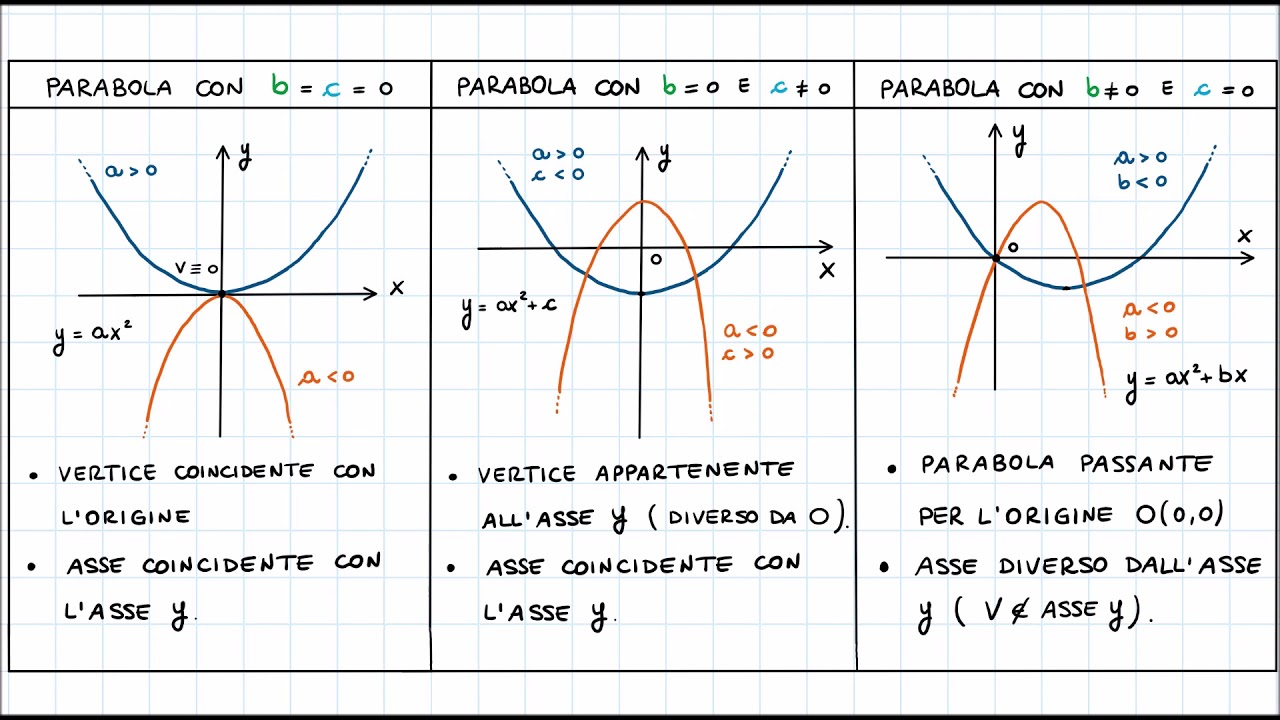
\includegraphics[width=\textwidth]{parabola.jpg}
        \end{center}
        $$ P_2(x) = ax^2 + bx + c, a \neq 0 $$
        $$ x^2 = c \Longrightarrow $$
        \begin{itemize}
            \item se $c > 0: x \pm \sqrt[2]{c} $
            \item se $c = 0: x = 0 $
            \item se $c < 0: \nexists x \in I\!R $
        \end{itemize}
        \newpage
        \subsubsection{Dimostrazione della correttezza della formula risolutiva per le equazioni di secondo grado}
            $$ ax^2 + bx + c = 0, a \neq 0 $$
            $$ a * \left[ x^2 + \frac{bx}{a} + \frac{c}{a} \right] = 0 $$
            $$ x^2 + \frac{bx}{a} + \frac{b^2}{4a^2} - \frac{b^2}{4a^2} + \frac{c}{a} = 0 $$
            $$ \left[ x + \frac{b}{2a} \right]^2 - \frac{b^2}{4a^2} + \frac{c}{a} = 0 $$
            $$ \left[ x + \frac{b}{2a} \right]^2 = \frac{b^2 - 4ac}{4a^2} $$
            $$ x + \frac{b}{2a} = \pm \sqrt[2]{\frac{b^2 - 4ac}{4a^2}} $$
            $$ x = -\frac{b}{2a} \pm \sqrt[2]{\frac{b^2 - 4ac}{4a^2}} $$
            $$ x = \frac{-b \pm \sqrt[2]{b^2 - 4ac}}{2a} $$
            In questa situazione abbiamo 3 opzioni:
            \begin{itemize}
                \item $b^2 - 4ac > 0 \Longleftrightarrow $ 2 soluzioni
                \item $b^2 -4ac = 0 \Longleftrightarrow $ 1 soluzione
                \item $b^2 - 4ac < 0 \Longleftrightarrow $ 0 soluzioni
            \end{itemize}
    \subsection{Modulo}
        $ |x| = \sqrt[2]{x^2} = $
        \begin{itemize}
            \item se $x > 0: x $
            \item se $x < 0: -x $
        \end{itemize}
        Geometricamente, il modulo è \textbf{la distanza} di x dal punto \textbf{0} sull'asse dei numeri $I\!R$. \\
        $$ |x| \leq a \Longleftrightarrow \left[ -a, a \right] $$
        $$ |x| \geq a \Longleftrightarrow \left( -\infty, -a \right] \cup \left[ a, +\infty \right) $$
        $$ -|x| \leq x \leq |x| $$ 
        \textbf{Disuguaglianza triangolare}: $|x + y| \leq |x| + |y|$
        $$ |x * y| = |x| * |y| $$
\section{Insiemi numerici}
    E' detta \textbf{insieme} una \textbf{collezione} di elementi per i quali è 
    sempre possibile rispondere alla domanda $x \in A$.
    \subsection{Applicazioni}
    Tramite un'applicazione, associo gli elementi dell'insieme A
    agli elementi dell'insieme B, detto \textbf{immagine} di A. \\
    Un'applicazione è:
    \begin{itemize}
        \item \textbf{Iniettiva}: $
            \forall x_1, x_2 \in A \textrm{ t.c. } x_1 \neq x_2:
            x_1 \rightarrow b_1 \neq x_2 \rightarrow b_2
        $
        \item \textbf{Suriettiva}: $\forall b \in B: 
            \exists a \in A \textrm{ t.c. } a \rightarrow b
        $
        \item \textbf{Biunivoca}: Suriettiva $\wedge$ Iniettiva
    \end{itemize}
    Se esiste un'applicazione suriettiva ed iniettiva fra $A$ e $B$ questi sono
    detti in \textbf{biezione}.
    \subsection{Definizione di $\mathbf{N}$ tramite gli insiemi}
    A questo punto possiamo definire i numeri naturali positivi partendo dagli insiemi.
    \begin{itemize}
        \item \textbf{0}: classe degli insiemi in biezione con $A = \emptyset$
        \item \textbf{1}: classe degli insiemi in biezione con $A = \{\emptyset\}$
        \item \textbf{2}: Classe degli insiemi in biezione con $A = \{\emptyset, \{\emptyset\}\}$
        \item \textbf{...}: ...
    \end{itemize}
    Possiamo accorgerci quindi come l'insieme $\mathbf{N}$ definisce la \textbf{cardinalità}
    degli insiemi. \\
    Da qui possiamo continuare:
    \begin{itemize}
        \item \textbf{$\mathbf{N} +$}: poichè $\mathbf{N}$ definisce la cardinalità degli insiemi,
            la somma di due numeri $\in \mathbf{N}$ è uguale alla cardinalità di 
            $(A \cup B) \forall A, B \textrm{ t.c. } A \cap B = \emptyset$.
        \item \textbf{-1}: quel numero t.c. $-1 + 1 = 0$. Da qui definiamo $\mathbf{Z}$.
        \item \textbf{$\frac{n}{m}$}: 
            $a_1, a_2, ..., a_n \in \mathbf{Z}, 0 \leq a_2, ..., a_n \leq 9:
            a_1 + \Sigma_{i=1}^{n}\frac{a^i}{10^i}$
        \item \textbf{$\mathbf{Q}$}: 
            ${\frac{n}{m},\frac{n_1}{m_1} \in \mathbf{Z}, m, m_1 \neq 0: 
            (n, m) = (n_1, m_1) \Longleftrightarrow (n * m_1) = (n_1 * m)}$. \\
            La struttura \textbf{periodica} è valida se si conviene che 
            $a,\overline{9} = a + 1$.
        \item \textbf{$\mathbf{Q} +$}: 
            $\frac{n}{m} + \frac{n_1}{m_1} = \frac{n * m_1 + m * n_1}{m * m_1}$
        \item \textbf{$\mathbf{Q} *$}:
            $\frac{n}{m} * \frac{n_1}{m_1} = \frac{n * n_1}{m * m_1}$
        \item \textbf{$\mathbf{Q}$ inverso}: 
            $\frac{n}{m} * \frac{n}{m}^{-1} = 1 \Longrightarrow 
            \frac{n}{m}^{-1} = \frac{m}{n}, n \neq 0$
        \item \textbf{$\mathbf{R}$}: {Tutti i numeri scritti in forma decimale
            anche con \textbf{infinite} cifre \textbf{non periodiche} dopo la virgola}
    \end{itemize}
    Possiamo infine definire le n-tuple di numeri $\left(a, b, ...\right)$ come
    \textbf{prodotto cartesiano} degli insiemi $A * B * ... = \{(a, b, ...) 
    \forall a \in A \wedge \forall b \in B \wedge ...\}$
    $$\mathbf{N} \subset \mathbf{Z} \subset \mathbf{Q} \subset \mathbf{R}$$
\section{Coefficiente binomiale}
    $$q \in R, q \neq 1 \Longrightarrow \Sigma_{k=0}^{n}q^k = \frac{1-q^{n+1}}{1-q} \Longleftrightarrow$$
    $$(1-q) * \Sigma_{k=0}^{n}q^k = 1-q^{n+1} \Longleftrightarrow$$
    $$\Sigma_{k=0}^{n}q^k - q * \Sigma_{k=0}^{n}q^k = 1-q^{n+1} \Longleftrightarrow$$
    $$\Sigma_{k=0}^{n}q^k - \Sigma_{k=1}^{n+1}q^k = 1 - q^{n+1} \Longleftrightarrow$$
    $$\left(\Sigma_{k=1}^{n}q^k + 1\right) - \left(\Sigma_{k=1}^{n}q^k + q^{n+1}\right) = 1 - q^{n+1} \Longleftrightarrow$$
    $$\Sigma_{k=1}^{n}q^k - \Sigma_{k=1}^{n}q^k + 1 - q^{n+1} = 1 - q^{n+1} \Longleftrightarrow$$
    $$\Sigma_{k=1}^{n}q^k = \Sigma_{k=1}^{n}q^k$$ 
    \\ \\
    $$\binom{n}{k} = \binom{n-1}{k-1} + \binom{n-1}{k} \Longleftrightarrow$$
    $$\frac{n!}{k!\left(n-k\right)!} = 
        \frac{\left(n-1\right)!}{\left(k-1\right)!\left(n-1-\left(k-1\right)\right)!} + \frac{\left(n-1\right)!}{k!\left(n-1-k\right)!} \Longleftrightarrow$$
    $$\frac{n!}{k!\left(n-k\right)!} = 
        \frac{\left(n-1\right)!}{\left(k-1\right)!\left(n-k\right)\left(n-k-1\right)!} + \frac{\left(n-1\right)!}{k\left(k-1\right)!\left(n-1-k\right)!} \Longleftrightarrow$$
    $$\frac{n!}{k!\left(n-k\right)!} = 
        \frac{k\left(n-1\right)! + \left(n-k\right)\left(n-1\right)!}{k!\left(n-k\right)!} \Longleftrightarrow$$
    $$\frac{n!}{k!\left(n-k\right)!} = 
        \frac{\left(n-1\right)!\left(k+n-k\right)!}{k!\left(n-k\right)!} \Longleftrightarrow$$
    $$\frac{n!}{k!\left(n-k\right)!} = \frac{n * \left(n-1\right)!}{k!\left(n-k\right)!} \Longleftrightarrow$$
    $$\frac{n!}{k!\left(n-k\right)!} = \frac{n!}{k!\left(n-k\right)!}$$
    \\ \\
    $$\left(a+b\right)^n = \Sigma_{k=0}^{n}\left(\binom{n}{k} * a^{n-k} * b^k\right)$$
    Dimostriamolo per induzione usando il seguente schema.
    \begin{enumerate}
        \item $P\left(n\right)$ è vera con $n=1$
        \item Supponiamo che $P\left(n\right)$ vera $\Longrightarrow P\left(n+1\right)$ vera
    \end{enumerate}
    Procediamo al primo passo:
    $$\left(a+b\right)^1 = \Sigma_{k=0}^{1}\left(\binom{1}{k} * a^{1-k} * b^k\right) \Longleftrightarrow$$
    $$a+b = \binom{1}{0} * a^1 * b^0 + \binom{1}{1} * a^{1-1} * b^1 \Longleftrightarrow$$
    $$a+b = 1 * a * 1 + 1 * 1 * b = a + b$$
    Abbiamo dimostrato che $P\left(1\right)$ è vera, procediamo quindi col secondo passaggio.
    $$\left(a+b\right)^{n+1} = \Sigma_{k=0}^{n+1}\left(\binom{n+1}{k} * a^{n+1-k} * b^k\right)$$
    $$\left(a+b\right)\left(a+b\right)^n = $$ 
    $$\left(a+b\right) * \Sigma_{k=0}^{n}\left(\binom{n}{k} * a^{n-k} * b^k\right) = $$
    $$\Sigma_{k=0}^{n}\left(\binom{n}{k} * a^{n+1-k} * b^k\right) + 
        \Sigma_{k=0}^{n}\left(\binom{n}{k} * a^{n-k} * b^{k+1}\right) = $$ 
    $$\Sigma_{k=0}^{n}\left(\binom{n}{k} * a^{n+1-k} * b^k\right) +  
        \Sigma_{k=1}^{n+1}\left(\binom{n}{k-1} * a^{n-k+1} * b^k\right) = $$ 
    $$\binom{n}{0} * a^{n+1} * b^0 + \Sigma_{k=1}^{n}\left(\binom{n}{k} * a^{n+1-k} * b^k\right) +
        \Sigma_{k=1}^{n}\left(\binom{n}{k-1} * a^{n-k+1} * b^k\right) + \binom{n}{n} * a^0 * b^{n+1} = $$
    $$a^{n+1} + 
        \Sigma_{k=1}^{n}\left[\left(\binom{n}{k} + \binom{n}{k-1}\right) * a^{n+1-k} * b^k\right]
        b^{n+1} = $$ 
    $$a^{n+1} + \Sigma_{k=1}^{n}\left(\binom{n+1}{k} * a^{n+1-k} * b^k\right) + b^{n+1} = $$
    $$\Sigma_{k=0}^{n+1}\left(\binom{n+1}{k} * a^{n+1-k} * b^{k}\right)$$
\section{Funzioni}
    \subsection{Definizione}
        Dati due insiemi $A$ e $B$, una funzione con \textbf{dominio} $A$ e 
        \textbf{codominio} B è una qualunque legge che \textbf{ad ogni} elemento
        di $A$ associa \textbf{uno ed uno solo} elemento di $B$.\\
        Può anche essere ad \textbf{n variabili} ed avere quindi n insiemi di partenza
        $$f: A \longrightarrow B \textrm{ t.c. } \forall x \in A \longrightarrow f(x) \in B$$
        Le funzioni \textbf{reali} a variabile \textbf{reale} sono le funzioni
        $$f: A \subset \mathbf{R} \longrightarrow \mathbf{R}$$
    \subsection{Immagine}
        $$ \{f(x) \forall x \in A\} \subset B $$
    \subsection{Grafico di una funzione}
        \subsubsection{Definizione}
            L'insieme dei punti $\mathbf{R}^2$ definiti da 
            $$ g_{\mathbf{R}} = \{(x,f(x)) \forall x \in A\}$$
        \subsubsection{Rappresentazione sul piano}
            Poichè $\mathbf{R}^2$ è rappresentabile sul piano cartesiano anche 
            $g_{\mathbf{R}}$ lo è
        \subsubsection{Proprietà fondamentale della funzione espressa col grafico}
        $$\forall x_0 \in A \, \exists!y_0 \textrm{ t.c. } {x = x_0} \cap {g_{\mathbf{R}}}
            = {(x_0, f(x_0))}$$
    \subsection{Proprietà delle funzioni}
        Una funzione è detta
        \begin{itemize}
            \item \textbf{pari}: $\forall x \in A: f(x) = f(-x)$
            \item \textbf{dispari}: $\forall x \in A: -f(x) = f(-x)$
            \item \textbf{limitata superiormente}: $\exists M \in \mathbf{R} 
                \textrm{ t.c. } M \geq f(x) \forall x \in A$
            \item \textbf{limitata inferiormente}: $\exists m \in \mathbf{R} 
                \textrm{ t.c. } m \leq f(x) \forall x \in A$
            \item \textbf{limitata}: $f(x)$ è limitata superiormente e inferiormente
            \item \textbf{monotona crescente in A}: $\forall x_1, x_2 \in A \textrm{ t.c. } 
                x_1 \leq x_2: f(x_1) \leq f(x_2)$
            \item \textbf{monotona decrescente in A}: $\forall x_1, x_2 \in A \textrm{ t.c. } 
                x_1 \leq x_2: f(x_1) \geq f(x_2)$
            \item \textbf{periodica di periodo T}: $\forall x \in A, x + kT \in A, 
                k \in \mathbf{Z}: f(x + kT) = f(x)$
            \item \textbf{successione}: il dominio è $\mathbf{N}$, $f(n) = a_n$
        \end{itemize}
    \subsection{Funzioni composte}
    \begin{itemize}
        \item $g(f(x)) = g \circ f(x)$
        \item \textbf{funzione neutra o identità}: $f(x) = x = I(x)$
        \item \textbf{funzione inversa}: $f \circ f^{-1}(x) = f^{-1} \circ f(x) = I(x)$
        \item $f$: Img$_{f^{-1}} \longrightarrow$ Def$_{f^{-1}}$
        \item $f^{-1}$: Img$_f \longrightarrow$ Def$_f$
        \item $f \circ f^{-1}$: Img$_f \longrightarrow$ Def$_f$
        \item $f^{-1} \circ f$: Img$_{f^{-1}} \longrightarrow$ Def$_{f^{-1}}$
    \end{itemize}
        \subsection{Condizioni di esistenza della funzione inversa}
            \begin{itemize}
                \item Img$_f \subset Def_g$ 
                \item f \textbf{iniettiva}: se, per assurdo, non lo fosse vorrebbe dire 
                    che $\exists x_1,x_2 \textrm{ t.c. } x_1 \neq x_2, \, \, y_1 = f(x_1) = f(x_2)$ e quindi
                    $f^{-1}(y)$ potrebbe essere sia $x_1$ che $x_2$, e quindi $f^{-1}$
                    non sarebbe una funzione
            \end{itemize}
    \subsection{Operazioni sui grafici}
        \begin{itemize}
            \item $f(x+k)$: spostamento a sx
            \item $f(x-k)$: spostamento a dx
            \item $f(x) + k$: spostamento in alto
            \item $f(x) - k$: spostamento in basso
            \item $-f(x)$: ribaltamento su asse y
            \item $(f(-x))$: ribaltamento su asse x
            \item $|f(x)|$: ribaltamento su asse y degli $y < 0$
            \item $f(|x|)$: Ribaltamento su asse x degli $x < 0$
        \end{itemize}
\section{Limiti}
    \subsection{Limiti convergenti}
        Una successione è detta \textbf{convergente} a $l$, o $\lim_{x \to \infty} = l$ se 
        $$\forall\epsilon > 0,\, \exists N = N\left(\epsilon\right) \textrm{ t.c. } \forall n > N \Longrightarrow
        |a_n - l| \leq \epsilon$$. \\
        Non tutte le successioni convergono.
    \subsection{Limiti divergenti}
        Una successione è detta \textbf{divergente} a $+\infty$, o 
        $\lim_{x \to \infty} = +\infty$, se $$\forall M > 0, \exists N = N\left(M\right)
        \textrm{ t.c. } \forall n > N \Longrightarrow a_n \geq M$$ e divergente a 
        $-\infty$ se $a \leq -M$.
        Non tutte le successioni divergono.
        \subsubsection{Convergenza per eccesso e per difetto}
            Una successione è detta tendere ad l per \textbf{eccesso} (l$^+$) nel caso 
            in cui a$_n$ > l, per \textbf{difetto}(l$^-$) in caso contrario.
            
    \subsection{Monotonia e limiti}
        Preso $A = \{a_n \forall n \in \mathbf{N}\}$, se $a_{n \in \mathbf{N}}$ è una successione \textbf{monotona}:
        \begin{itemize}
            \item \textbf{crescente}: converge a sup$_A$ se limitata, se no diverge a $+\infty$
            \item \textbf{decrescente}: converge ad inf$_A$ se limitata, se no diverge a $-\infty$
        \end{itemize}
    \subsection{Esempi di successioni limitate}
        $$\lim_{n \to \infty} \frac{1}{n} = 0$$ 
        $$\Longrightarrow |\frac{1}{N}-0| \leq \epsilon \Longrightarrow \frac{1}{\epsilon} \leq n$$
        $$\Longrightarrow \textrm{ per } N = \frac{1}{\epsilon} \textrm{ esiste sempre } n > N$$
        \\
        $$\lim_{n \to \infty} 2^n = \infty$$
        $$\Longrightarrow 2^n \geq M \Longrightarrow n \geq \log_2M$$
        $$\Longrightarrow \textrm{ per } N = \log_2M \textrm{ esiste sempre } n > log_2M$$ 
        \\
        $$\lim{n \to \infty} \frac{n+1}{n-1} = 1$$
        $$\Longrightarrow |\frac{n+1}{n-1} - 1| \leq \epsilon \Longrightarrow \geq -\epsilon \, \forall n \in \mathbf{N}$$
        $$\Longrightarrow \frac{n+1}{n-1} < 1 + \epsilon \Longrightarrow n+1 \leq n + n\epsilon -1 - \epsilon$$
        $$\Longrightarrow 2 + \epsilon \leq n\epsilon \Longrightarrow n \geq \frac{2}{\epsilon} + 1$$
    \subsection{Algebra dei limiti}
        $\lim_{n \to n_0} a_n = a \, \, \lim_{n to \infty} b_n = b$ \\
        $\lim_{n \to n_0} a_n + b_n = a + b$ \\
        $\lim_{n \to n_0} a_n * b_n = a * b$ \\
        $\lim_{n \to n_0} a_n^{b_n} = a^b$ \\
        $\lim_{n \to n_0} f(a_n) = f(a)$ \\
    \subsection{Teorema di permanenza del segno}
        $\lim_{n \to n_0} a_n = a, \, a \geq 0 \Longrightarrow \exists N \in \mathbf{N} \textrm{ t.c. }
            \forall n > N: a_n \geq 0$ \\
        $\lim_{n \to n_0} a_n = a, \, a \leq 0 \Longrightarrow \exists N \in \mathbf{N} \textrm{ t.c. }
            \forall n > N: a_n \leq 0$ \\
        E' quindi implicato: \\
        $\lim_{n \to n_0} a_n = a, \, \lim_{n \to n_0} b_n = b, \, a_n > b_n \Longrightarrow a > b$
    \subsection{Teorema dei carabinieri}
        $a_n \leq b_n \leq c_n$
        $a = c \Longrightarrow a = b = c$
        



\end{document}


